\documentclass{article}
\usepackage{tikz}
\usetikzlibrary{shapes.geometric, arrows.meta, positioning, fit, backgrounds, calc}
\begin{document}

\begin{figure}[h]
\centering
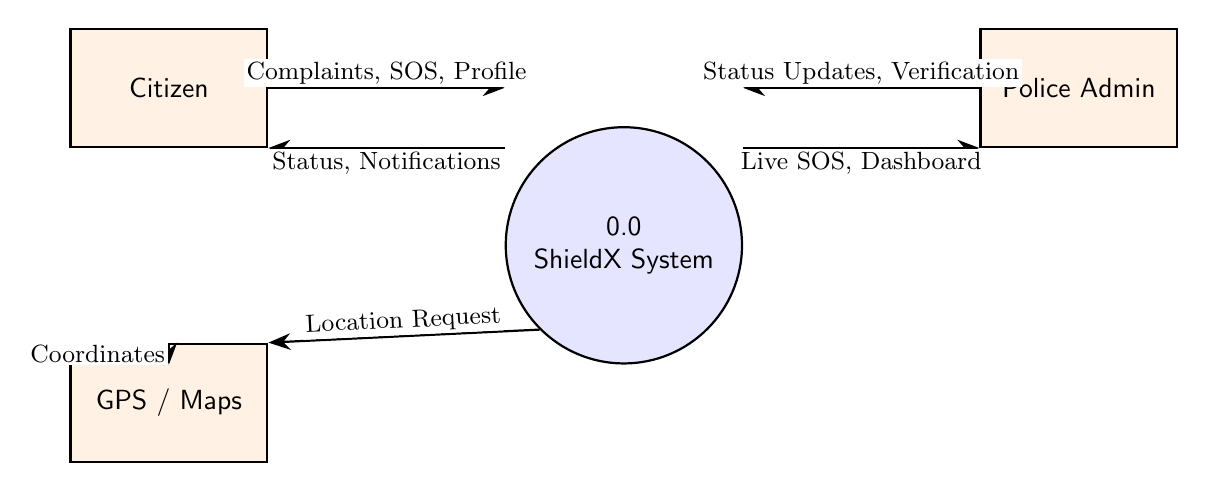
\begin{tikzpicture}[
    node distance=2cm and 3cm,
    every node/.style={font=\sffamily},
    process/.style={circle, draw=black, thick, minimum size=3cm, text centered, text width=2.5cm, fill=blue!10},
    entity/.style={rectangle, draw=black, thick, minimum width=2.5cm, minimum height=1.5cm, text centered, fill=orange!10},
    arrow/.style={-{Stealth[scale=1.2]}, thick},
    label/.style={font=\small, align=center, fill=white, inner sep=1pt}
]

% Level 0
\node[process] (system) {0.0 \\ ShieldX System};
\node[entity, left=of system, yshift=2cm] (citizen) {Citizen};
\node[entity, right=of system, yshift=2cm] (admin) {Police Admin};
\node[entity, left=of system, yshift=-2cm] (gps) {GPS / Maps};

\draw[arrow] (citizen.east) -- node[above, label, sloped] {Complaints, SOS, Profile} (system.west |- citizen.east);
\draw[arrow] (system.west |- citizen.south east) -- node[below, label, sloped] {Status, Notifications} (citizen.south east);

\draw[arrow] (admin.west) -- node[above, label, sloped] {Status Updates, Verification} (system.east |- admin.west);
\draw[arrow] (system.east |- admin.south west) -- node[below, label, sloped] {Live SOS, Dashboard} (admin.south west);

\draw[arrow] (system.south west) -- node[above, label, sloped] {Location Request} (gps.north east);
\draw[arrow] (gps.north) -- node[left, label] {Coordinates} (system.south -| gps.north);

\end{tikzpicture}
\end{figure}

\end{document}